\documentclass[12pt,onecolumn,a4paper,fleqn]{article}
\usepackage[top=1in, bottom=1in, left=0.75in, right=0.75in]{geometry}
\usepackage{epsfig,graphicx,subfigure,amsthm,amsmath}
\usepackage[table,xcdraw,svgnames]{xcolor}
\usepackage{setspace}
\usepackage{mathtools}
\usepackage{fancyhdr}
\usepackage{sidecap}
\usepackage{tikz}
\usepackage{pgfplots}
\usetikzlibrary{decorations.pathreplacing}
\usepackage{relsize}
\usepackage{color,xcolor}
\usepackage[framed,numbered]{matlab-prettifier}
\usepackage{float}
\usepackage{enumerate}
\usepackage{booktabs}
\usepackage{setspace}
\usepackage{datetime}
\usepackage{xepersian}


\settextfont[Path=fonts/,BoldFont={ZarBd.ttf},BoldFeatures={Scale=0.9}]{BZar.ttf}

%\DeclarePairedDelimiter\ceil{\lceil}{\rceil}
%\DeclarePairedDelimiter\floor{\lfloor}{\rfloor}

\definecolor{vgreen}{RGB}{104,180,104}
\definecolor{vblue}{RGB}{49,49,255}
\definecolor{vorange}{RGB}{255,143,102}

\pagestyle{fancy}
\fancyhf{}
\rhead{\textbf{آزمایشگاه طراحی سیستم‌های دیجیتال}}
\chead{\textbf{گزارش آزمایش سوم}}
\lhead{\textbf{\nouppercase{\rightmark}}}
\cfoot{({\thepage})}
\renewcommand{\headrulewidth}{1pt}
\renewcommand{\footrulewidth}{1pt}
\renewcommand{\sectionmark}[1]{\markright{#1}}
\renewcommand{\subsectionmark}[1]{\markright{#1}}
%\newdateformat{monthyeardate}{%
%	\monthname[\THEMONTH], \THEYEAR}

\onehalfspacing
\begin{document}
	%%% title pages
	\large
	\begin{titlepage}
		
		\begin{center}
			\begin{huge}
				\textbf{
					به نام خدا\\
				}
			\end{huge}
			
			\vspace*{1.5cm}
			
\includegraphics[scale=0.9]{source/sharif_logo.png}\\
			\vspace*{0.5cm}
			\begin{Large}
				
				دانشگاه صنعتی شریف\\
				\vspace*{0.25cm}
				\textbf{
					دانشکده مهندسی کامپیوتر\\
				}
			\end{Large}
			\vspace*{3cm}
			\begin{huge}
				\textbf{
					آزمایشگاه طراحی سیستم‌های دیجیتال\\
					\vspace*{1.75cm}
				}
			\end{huge}
			
			\begin{Large}
				\textbf{
					آزمایش سوم:\\
					طراحی مقایسه‌کننده باینری به صورت ترکیبی و ترتیبی\\
				}
			\end{Large}
			
			\noindent\rule[1ex]{\linewidth}{1pt}
			\vspace*{1.5cm}
			\begin{Large}
				محمدجواد هزاره، یاسین موسوی
				
				\vspace*{1.5cm}
				%					\textbf{\today}
				\textbf{
					تابستان 1400
				}
			\end{Large}			
		\end{center}
		\thispagestyle{empty}
	\end{titlepage}	
	\pagebreak
	
	\tableofcontents
	\thispagestyle{empty}
	\pagebreak
	\section{مقدمه}
	\subsection{شرح آزمایش}
	در این آزمایش هدف طراجی یک مقايسه‌کننده باینری هم به صورت ترکیبی و هم به صورت ترتیبی است. طراجی با استفاده از زبان
	\lr{verilog}
	 و به شکل توصیف جریان داده صورت گرفته است.
	\pagebreak
	\section{مدار ترکیبی}
	\subsection{رابط‌ کاربری}
	رابط کاربری مدار ترکیبی بسیار ساده بوده و شامل دو ورودی چهار بیتی
	\lr{A}
	و
	\lr{B}
	می‌شود. خروجی مدار نیز سه سیگنال 
	\lr{eq}،
	\lr{gt}
	و
	\lr{lt}
	را در بر می‌گیرد که فعال خواهند بود اگر به ترتیب ورودی‌ها با یکدیگر برابر باشند، یا ورودی 
	\lr{A}
	بزرگ‌تر از ورودی 
	\lr{B}
	باشد و یا ورودی
	\lr{A}
	کوچک‌تر از ورودی 
	\lr{B}
	باشد.
	\begin{figure}[H]
		\centering
		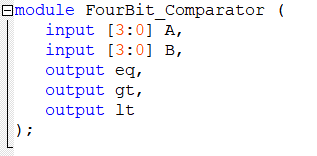
\includegraphics[scale=0.95]{source/interface_comb.png}
		\caption{رابط کاربری مدار ترکیبی}
	\end{figure}
	\subsection{نحوه کار}
	برای پیاده‌سازی مدار نیز از واحد مقايسه‌کننده یک بیتی استفاده شده و چهار عدد از این مقايسه‌کننده‌ها پشت‌سر یکدیگر استفاده شده‌اند.
	\subsection{شبیه‌سازی}
	\pagebreak
	\section{مدار ترتیبی}
	\subsection{رابط کاربری}
	\subsection{نحوه کار}
	\subsection{شبیه‌سازی}
\end{document}